\documentclass{beamer}
\usetheme{SimplePlus}

% Packages pour améliorer les mathématiques
\usepackage[utf8]{inputenc}
\usepackage{textcomp}
\usepackage{amsmath}
\usepackage{amssymb}
\usepackage{mathtools}
\usepackage{xcolor}
\usepackage{svg}
\usepackage{tikz}
\usepackage{esvect}
\usepackage{pgfplots}
\usepackage[european]{circuitikz}
\usepackage{siunitx}

\pgfplotsset{compat=1.18}

\usetikzlibrary{%
  decorations.pathmorphing,   % pour ressorts et ondulations
  shapes,                     % formes prédéfinies
  calc,                       % calcul de coordonnées
  arrows.meta,                % flèches modernes
  positioning,                 % positionnement relatif
  patterns
}

\tikzset{
  spring/.style={
    decorate,
    decoration={coil, segment length=6pt, amplitude=3pt, post length=4pt, pre length=4pt}
  },
  masspoint/.style={
    circle,
    minimum size=4mm,
    inner sep=0pt,
    draw=none,
    path picture={
      \draw[line width=1pt]
        ($(path picture bounding box.center)+(-1.2mm,-1.2mm)$)
        --
        ($(path picture bounding box.center)+(1.2mm,1.2mm)$);
      \draw[line width=1pt]
        ($(path picture bounding box.center)+(-1.2mm,1.2mm)$)
        --
        ($(path picture bounding box.center)+(1.2mm,-1.2mm)$);
    }
  },
}
\tikzstyle{ground}=[preaction={fill,top color=black!10,bottom color=black!5,shading angle=20},
                    fill,pattern=north east lines,draw=none,minimum width=0.3,minimum height=0.6]



\usefonttheme[onlymath]{serif}

\title{Microscopie à Force Magnétique}
\author{Rafael Martinez}
\date{\today}

% Redéfinir le pied de page avv les éléments spécifiés
\setbeamertemplate{footline}{
  \ifnum\value{framenumber}>1 % Vérifie si le numéro de la diapositive est supérieur à 1
    \leavevmode%
    \hbox{%
    \begin{beamercolorbox}[wd=.25\paperwidth,ht=2.25ex,dp=1ex,center]{author in head/foot}%
      \usebeamerfont{author in head/foot} Rafael Martinez
    \end{beamercolorbox}%
    \begin{beamercolorbox}[wd=.5\paperwidth,ht=2.25ex,dp=1ex,center]{title in head/foot}%
      \usebeamerfont{title in head/foot} Microscopie à Force Magnétique
    \end{beamercolorbox}%
    \begin{beamercolorbox}[wd=.25\paperwidth,ht=2.25ex,dp=1ex,center]{date in head/foot}%
      \usebeamerfont{date in head/foot}Candidat 22990 \hfill
      \ifnum\value{framenumber}<31
        \textbf{\insertframenumber{/30}}
      \else
        \textbf{\insertframenumber{}/\pageref{LastPage}}
      \fi
    \end{beamercolorbox}}%
    \vskip0pt%
  \fi
}


\begin{document}

\frame{\titlepage}

\begin{frame}{Plan}
    \tableofcontents
\end{frame}

\section{Le microscope à force magnétique}

\begin{frame}{Principe de fonctionnement}
    \begin{figure}
        \centering
        \includegraphics[width=0.95\linewidth]{static/mfm.jpg}
    \end{figure}
\end{frame}

% \begin{frame}{Caractéristiques}
%     \begin{itemize}
%         \item Capacité à imager des échantillons non conducteurs
%         \item Résolution élevée: 10 nm
%         \item Nombreux modes de fonctionnement
%         \begin{itemize}
%             \item Contact
%             \item Non contact
%             \item Mode dynamique
%         \end{itemize}
%     \end{itemize}
% \end{frame}

\begin{frame}{Modèle de la poutre encastrée statique}
    \begin{columns}
        \begin{column}{0.4\textwidth}
            \begin{figure}
                \centering
                \includegraphics[width=\linewidth]{static/poutre.png}
            \end{figure}
        \end{column}
        \begin{column}{0.3\textwidth}
            \begin{figure}
                \centering
                \includegraphics[width=\linewidth]{static/ressort_amortit.jpg}
            \end{figure}
        \end{column}
    \end{columns}

    % petit espace
    \vspace{0.5cm}
    Équivalent au système masse-ressort-amortisseur:

    \[
    \vv F_{el} = -k x \vv{u_x} \qquad  \vv f_{m} = -\alpha \frac{dx}{dt} \vv {u_x}
    \]

    \begin{equation}\label{eq:diffeq}
        m x''(t) + \alpha x'(t) + k x(t) = 0
    \end{equation}

    % \[
    % \underline x(t) = \underline X_h \exp{\left(\left[-\frac{\omega_0}{2Q} + i\omega_0 \sqrt{\frac{1}{4Q^2} - 1}\right]t\right)}
    % \]

    % omega/Q  = alpha/m
    % Q = 
\end{frame}


\begin{frame}{Ajout de l'aimant}

    \begin{columns}
    \begin{column}{0.5\textwidth}
        L'interaction pointe échantillion s'exprime:
        \[
            \vv{F_{mag}} = \vv m_p \cdot \vv{\mathrm{grad}} \vv{B}_{e}
        \]

        
        % \begin{equation}    
        \[      
            mx''(t) + \alpha x'(t) + k x(t) = F_{mag}(x)
        \]

        En statique:

        \[
            % x(t) = x_0 +\frac{m_p}{k}\frac{\partial B_e}{\partial x}
            \boxed{
            x_{eq} = \frac{F_{mag}(x_{eq})}{k}
            }
        \]

        Mesure directe de $F_{mag}$.
    \end{column}
    \begin{column}{0.5\textwidth}
        % \begin{itemize}
            Pointe magnétique de moment $\vv{m_p}$
            Échantillon magnétique $\vv{B}_{e}$
        % \end{itemize}
        \begin{center}
            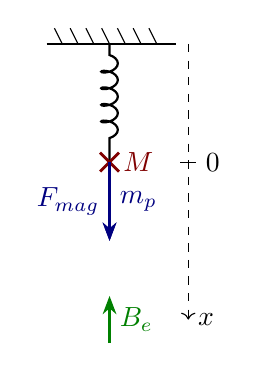
\begin{tikzpicture}

            % Axe x
            \draw[->, dashed] (1,0) -- (1,-3.5) node[right] {$x$};
            \draw[] (0.90,-1.5) -- (1.1,-1.5)
                node[midway, right=0.1] {$0$};

            % % Dampner \alpha line, open box line
            % \draw[thick] (-0.8,0) -- (-0.8,-0.5);

            % Support
            \draw[thick] (-0.8,0) -- (0.85,0);
            \foreach \x in {-0.6,-0.4,...,0.8}
            \draw (\x,0) -- (\x-0.1,0.2);
            % \draw[ground] (-\W/2,0) rectangle++ (\W,-\D);
            % \draw[ground] (-0.5,0) rectangle++ (1,0.2);

            % Ressort
            \draw[spring, thick] (0,0) -- (0,-1.5);

            % Masse
            \node[masspoint, red!50!black] at (0,-1.5) {}
                node[right, red!50!black] at (0.05,-1.5) {$M$};

            % Pointe
            \draw[-{Stealth}, thick, blue!50!black] (0, -1.5) -- (0,-2.5)
            node[midway, right] {$\vv{m_p}$};
            \draw[-{Stealth}, thick, blue!50!black] (0, -1.5) -- (0,-2.5)
            node[midway, left] {$\vv{F_{mag}}$};

            % --- Aimant ---
            % \node[draw, rectangle, minimum width=0.6cm, minimum height=1cm]
            % at (0,-3.5) {};
            \draw[-{Stealth}, thick, green!50!black] (0,-3.8) -- (0,-3.2)
            node[midway, right] {$\vv{B}_{e}$};

            \end{tikzpicture}
        \end{center}
    \end{column}
\end{columns}
\end{frame}

\begin{frame}{}
    En dynamique, proche de l'équilibre $x\simeq x_{eq}$, on fait l'approximation suivante:
    \[
    F_{mag}(x) = F_{mag}(x_{eq}) + \frac{\partial F_{mag}}{\partial x}\bigg|_{x_{eq}} (x - x_{eq})
    \]

    Equation différentielle linéarisée:
    \[
    m x''(t) + \alpha x'(t) + \left(k-\frac{\partial F_{mag}}{\partial x}\bigg|_{x_{eq}}\right) x(t) = c_1
    \]

    Raideur effective:

    \[
    \boxed{k_{eff} = k - \frac{\partial F_{mag}}{\partial x}\bigg|_{x=x_{eq}}}
    \]

\end{frame}

\begin{frame}{Analyse des solutions}
    Solution homogène:
    % \[
    % \underline x(t) = \underline X_h \exp{\left(\left[-\frac{\omega_0}{2Q} + i\omega_0 \sqrt{\frac{1}{4Q^2} - 1}\right]t\right)}
    % \]
    \[
    \underline x(t) = \underline X_h e^{(r+i\Omega)t} \qquad
    \]

    % \[
    % r = -\frac{\omega_0}{2Q} = -\frac{\alpha}{2m} \qquad \Omega = \omega_0 \sqrt{\frac{1}{4Q^2} - 1} = \sqrt{\frac{\alpha^2}{4m^2} - \frac{k_{e}}{m}}
    % \]
    \[
    r = -\frac{\omega_0}{2Q} = -\frac{\alpha}{2m} \qquad \Omega = \sqrt{\frac{\alpha^2}{4m^2} - \frac{k_{e}}{m}}
    \]

    \begin{columns}
    \begin{column}{0.5\textwidth}
    Transformée de fourier:
        \[
        \underline{\tilde{x}}(\omega) = \int_{0}^{+\infty} \underline x(t) e^{-i\omega t} dt
        \]

        % \[
        % \underline x(\omega) = \frac{\underline X_h}{-\frac{\omega_0}{2Q} + i\left(\omega_0 \sqrt{\frac{1}{4Q^2} - 1} - \omega\right)}
        % \]

        % \[
        % \underline x(\omega) = \frac{\underline X_h}{-r-i(\Omega - \omega)}
        % \]

        \[
            \left|\frac{\underline x(\omega)}{\underline X_h}\right|^2 = \frac{1}{\left(-r\right)^2 + \left(\Omega - \omega\right)^2}
        \]
    \end{column}
    \begin{column}{0.35\textwidth}
        \begin{figure}
            \centering
            \includegraphics[width=\linewidth]{static/lorentz.jpg}
        \end{figure}
    \end{column}
        
    \end{columns}

    % amplitude / np.sqrt(1 + ((x - f0) / (df / 2)) ** 2)

    % \[
    % |\underline x(\omega)| = \frac{|\underline X_h|}{\sqrt{\left(-\frac{\omega_0}{2Q}\right)^2 + \left(\omega_0 \sqrt{\frac{1}{4Q^2} - 1} - \omega\right)^2}} = \frac{A}{}
    % \]
\end{frame}

% \begin{frame}{Résultats expérimentaux}
%     Règle sans masse ajoutée, régime transitoire libre.

%     Prise vidéo 200 images par seconde, pointage python OpenCV.

%     \begin{columns}
%         \begin{column}{0.5\textwidth}
%             \begin{figure}
%                 \centering
%                 \includegraphics[width=\linewidth]{static/libre-s.png}
%             \end{figure}
%         \end{column}
%         \begin{column}{0.5\textwidth}
%             \begin{figure}
%                 \centering
%                 \includegraphics[width=\linewidth]{static/montage1.png}
%             \end{figure}
%         \end{column}
%     \end{columns}
% \end{frame}


\begin{frame}{Oscillation forcée}
    Force d'excitation harmonique:
    \[
    F(t) = F_0 \cos(\omega t)
    \]

    Equation différentielle associée:
    \[
    \underline {x}''(t) + \frac{\omega_0}{Q} \underline {x}'(t) + \omega_0^2 \underline {x}(t) = F_0 e^{i\omega t} \qquad \omega_0^2 = \frac{k_{e}}{m}
    \]

    Solution particulière:

    \begin{columns}
        \begin{column}{0.5\textwidth}

    \[
    \underline x_p(t) = X_m e^{i(\omega t + \varphi_p)}
    \]
    \[
    \underline{X_m} = \frac{F_0}{\omega_0^2 - \omega^2 + i\frac{\omega_0 \omega}{Q}}
    \]

    \[
    \varphi_p(\omega) = \tan^{-1}\left(-\frac{\omega \omega_0 / Q}{\omega_0^2 - \omega^2}\right)
    \]
        \end{column}
        \begin{column}{0.5\textwidth}
            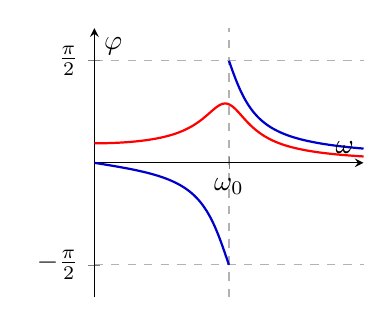
\begin{tikzpicture}
            \begin{axis}[
                width=5cm, height=5cm,
                domain=0:2,
                samples=200,
                axis lines=middle,
                grid=both,
                grid style={dashed, gray!60},
                xmin=0, xmax=2,
                ymin=-pi/2-0.5, ymax=pi/2+0.5,
                xtick={0,1},
                xticklabels={$0$,$\omega_0$},
                ytick={-pi/2,0,pi/2},
                yticklabels={$-\frac{\pi}{2}$,$0$,$\frac{\pi}{2}$},
                xlabel={$\omega$},
                ylabel={$\varphi$},
            ]
            \addplot[mark=none, domain=0:0.9999, blue!80!black, thick] 
                {atan(-(x)/(3*(1-x^2))) * pi/180};

            \addplot[mark=none, domain=1.0001:2, blue!80!black, thick] 
                {atan(-(x)/(3*(1-x^2))) * pi/180};

            % 

            \addplot[mark=none, red, thick] {0.3 / sqrt((1-x^2)^2+(x/3)^2)};

            \end{axis}
            \end{tikzpicture}
        \end{column}
    \end{columns}
\end{frame}

\frame{\frametitle{Interprétation du déphasage}
    En présence d'un champ et pour $\omega \approx \omega_0$:

    \[
    \varphi(\omega_0) = \tan^{-1}\left(\frac{k}{Q\frac{\partial F_{mag}}{\partial x}}\right)
    \]


    On déduit:

    \[
    \Delta \varphi(\omega_0) \approx \frac Qk \frac {\partial F_{mag}}{\partial x}
    \]

    (A démontrer).
}

\section{Mise en oeuvre expérimentale du levier}

\frame{\frametitle{Premier dispositif}
    \begin{columns}
        \begin{column}{0.45\textwidth}
            \begin{figure}
                \centering
                \includegraphics[width=\linewidth]{static/exp_01.jpg}
            \end{figure}
        \end{column}
        \begin{column}{0.25\textwidth}
            \begin{figure}
                \centering
                \includegraphics[width=\linewidth]{static/modele_1.png}
            \end{figure}
        \end{column}
    \end{columns}

    Bobine de fil de cuivre (200 tours).

    Levier en fer (baton de ramoneur)

    \[ k= \qquad Q= \qquad f_0 =\]

}

\begin{frame}
    \frametitle{Captation}

    \begin{columns}
        \begin{column}{0.5\textwidth}
            \begin{figure}
                \centering
                \includegraphics[width=\linewidth]{static/pdt-photo.png}
            \end{figure}
        \end{column}
        \begin{column}{0.5\textwidth}
            \begin{figure}
                \centering
                \includegraphics[width=\linewidth]{static/exp_02.jpg}
            \end{figure}
        \end{column}
    \end{columns}
\end{frame}
\end{document}
